\chapter{Background and Related Work}
\label{cha:theory}

To be able to grasp the concept of how HTTP-adaptive streaming (HAS) and geo-based streaming (GBS) works we first present a background on HAS and GBS in order to further strengthen our methodology and the interpretation of our result. Since we are using HAS and GBS when programming our interface there is a need to study existing works and articles. This knowledge is essential to be able to implement an upgraded media player that is adapted to streaming and seemlessly switching between videos from different geographical positions.

There are many related works to our project. Many of these works are focusing on branching videos in media players, which describes ways to allow for users to seamlessly switch between videos without quality degradation or interruptions \cite{qualbranch, hasmultipath,scalableOnDemand}. Zhao et al. \cite{scalableOnDemand} propose protocols that enables the possibility of scaleable on-demand content with minimal server load and developing a way that limits the lower bound bandwidth requirement using multicast \cite{scalableOnDemand}. Other works talks about policies for providing a good way of prefetching several videos in different ways, providing means of allowing prefetching and instantaneous playback without playback quality degradation. The work studies the off-periods observed in HAS-players to utilize it as effectively as possible \cite{bandawarePrefetch}. There are also works that have looked at optimiziation of video quality by observing and controlling the playback buffer by in turn looking at the network capacity, providing an algorithm for optimizing the video quality without any unnecessary buffering \cite{bufferbased}.

Some works have dwelved more into how to prefetch in an effective way. Khemmarat et al. \cite{watchingprefetching} have looked at different ways to prefetch videos in-order to allow for the best user experience. While watching a Youtube video, the user experience is significantly increased when the time the video is paused and buffering is minimal. They provide an approach that tries to predict which video a user will click and and prefetch it. By looking at three different schemes they found that by combining caching and prefetching the hit-ratio, for which a clicked video is prebuffered, would increase up to 80 \%. Their proposed schemes improves video playback in a way that it avoids playback delay. The trade-off of a higher bandwidth usage is minimized when combinding prefetching and caching of videos and by not having large amount of videos to prefetch. If this were to be combined in some way with what we want to accomplish with prefetching in the future then it will allow for a much better video experience.

\section{HTTP-based Adaptive Streaming}
\label{sec:has}

Mobile users streaming media sometimes suffers from playback interruption when faced with a bad wireless connection. HTTP-adaptive streaming seeks to resolve this by dynamically changing the bitrate and therefore quality of the stream to make do with the connection that is available to the user. To ensure smooth transitions between these quality swaps HAS also tries to predict the swaps in advance using various methods depending on the HAS framework. There are many algorithms for these predictions, but a brief example would be to use previous logged connectivity history and future connectivity using geo-based methods to make predictions \cite{gtube}. Most HAS players uses weighted average of past download time/rates in order to estimate download rate of available bandwidth \cite{qualbranch}. With these HAS predictions, a stream quality fitting the user’s network quality can be buffered \cite{gtube}.

By implementing HAS into our interface we need to prefetch data from several close-by video streams at the recording area (if not all, depending on number of them) and build up a small enough buffer that makes switching between these different streams seamless. By looking at how HAS is used when implementing an interactive branched video we can say that parallel TCP connections are a must in-order to achieve this with the cost of wasting bandwidth and lower playback quality. This depends mainly on the number of videos that needs to be prefetched. Most HAS video players has a cap on the buffer size in order to avoid wasting bandwidth. Krishnamoorthi et al. \cite{qualbranch} use a customized HAS player that solves the problem of trade-off between quality and number of chunks downloaded. The playback chunks are stored in the playback buffer while the prefetched chunks are stored in a browser cache thus allowing those chunks to be retrieved quickly. This ensures that no playback interruption occurs for the user. The way they download the chunks are done in a round-robin way to ensure that a buffer workahead is built up enough for seamless playback in parallel TCP downloading. 

Downloading chunks in a round-robin way is how we plan chunks will be downloaded in our media player. This method will be used together with the idea of prefetching in the downtime of a HAS-player. Most HAS-players has some kind of buffer treshold $T_{max}$ where downloading is interrupted when reached and will resume only when the minimum buffer $T_{min}$ is reached. This kind of behaviour can be called an \textit{on-off behaviour} which can lead to poor performance under conditions with competing traffic. It is common in several HAS-players like Netflix and Microsoft Smooth Streaming for example \cite{bandawarePrefetch}. Krishnamoorthi et al. \cite{bandawarePrefetch} provide policies and ideas that reduce the start-up time of videos by an order of magnitude and ensures the highest possible playback quality to be viewed. A way of improved channel utilization that allows for instantaneous playback of prefetched videos. They provide an HAS solution which we will take advantage of together with prefetching nearby streams in a round-robin way. The solution allows for prefetching and buffer management in such a way that videos can be downloaded parallel and switched to instantaneously without interrupting the user experience. By using a novel system to utilize the unused bandwidth during off periods this allows for videos to simultaneously be prefetched while maintaining a fair bandwidth share. It also increases the playback quality in which a video is downloaded \cite{bandawarePrefetch}. This idea will be discussed further in section 2.2 when we describe our idea of downloading streams.

There can occur several problems in HAS players \cite{qualbranch}. Huang et al. \cite{streamrate} show that when a competing TCP flow starts a so called “downward spiral effect” occurs and the downgrade in throughput and playback rate becomes severe. This is caused by a timeout in the TCP congestion window, high packet loss in competing flows and when a client has a lower throughput. Then the playback rate is lower due to smaller buffer segments which makes a video flow more susceptible to perceiving lower throughput and thus creating a spiral. A possible solution is to have larger segment size and by having an algorithm which is less conservative, meaning that requesting a video at lower rate than it's perceived. This is something that we can keep in mind since quality can decrease drastically when having several videos buffering in parallel, though we will not have to buffer a full video at the same time but only chunks of a video while the main stream is being watched.

\section{Non-linear Streaming and Multipath}
\label{sec:nonlinear}

Krishnamoorthi et al. \cite{hasmultipath} use the technique of storing prefetched chunks in a playback buffer simliar to [6]. Prefetching for different branches to allow seamless switching between videos, using the notion of multi-path nonlinear videos to stitch together videos using a novel buffer management and prefetching policy. This prefetching decreases the time it takes to switch between branches considerably and is something we will take advantage of since the code we use from Krishnamoorthi et al.\cite{qualbranch} are based on a similar policy \cite{hasmultipath}. If we look at what Zhao et al. \cite{scalableOnDemand} wrote they describe how choosing a correct branching point sufficiently ahead of time with an accuracy of 75 \% greatly reduces bandwidth requirements by requesting nonlinear video content where chunks are downloaded in parallel without causing jitter. This is something which is really efficient and important for users that would like the ability to switch between different videos on-demand. Selecting what type of chunks should be downloaded is hard to accomplish, atleast on a broader context when considering watching TV stream during TV broadcasting \cite{scalableOnDemand}. Most of these works are mostly focused on branching videos which is simliar but not entirely simliar to what we will be doing \cite{qualbranch, hasmultipath,scalableOnDemand}. We will contribute more to the possibility of prefetching several videos parallel and then be able to switch to any of  them on-demand. However the ideas used when handling branching videos is something that will be used in our mediaplayer.

Figure \ref{fig:HAS1} and \ref{fig:HAS2} illustrate an example of a stream consisting of chunks being played, how these chunks are prefetched and stored and a swap between two streams.

\begin{figure}[!ht]
\begin{center}
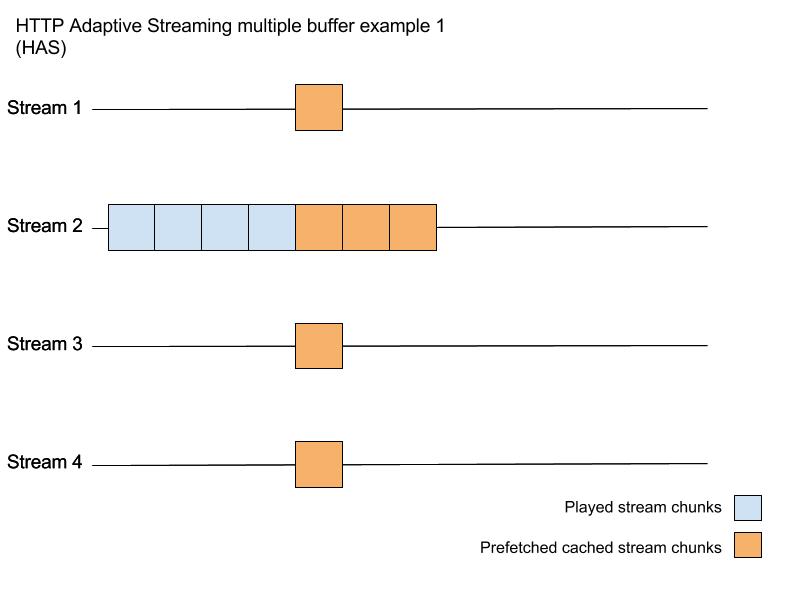
\includegraphics[scale=0.4]{HAS1.png}
\caption{HAS Parallell Stream Buffer 1}
\label{fig:HAS1}
\end{center}
\end{figure}

\begin{figure}[!ht]
\begin{center}
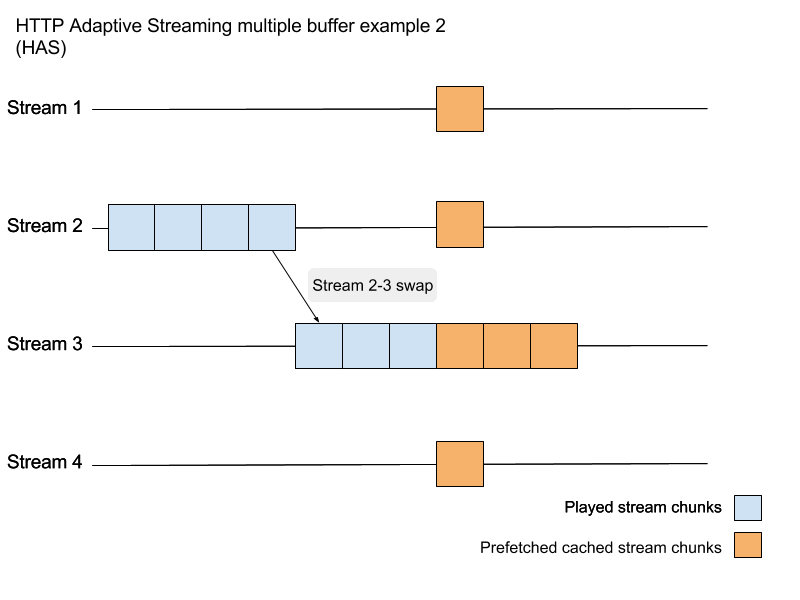
\includegraphics[scale=0.4]{HAS2.png}
\caption{HAS Parallell Stream Buffer 2}
\label{fig:HAS2}
\end{center}
\end{figure}

There have been works that have looked at a way of optimizing periodic broadcast delivery for non-linear media, by creating functions and an algorithms that provides a way to effectively control over quality of service for clients with varying playback paths. They then look at cases were clients makes a path selection at their arrival instance over branching tree paths and graphs.\cite{optimizedbroadcast}


\section{Strobe Media Playback}
\label{sec:smp}

To display the stream in our application we will be using a media player called Strobe Media Playback (SMP), created with the Open Source Media Framework (OSMF) by Adobe Systems. The OSMF itself is build upon Adobe Flash Player, while becoming more outdated by day and discontinued by some, is widely used for media and other graphic applications and suffices to use for the proof-of-concept of our application. In practice this means that the media player is created using the tools that OSMF provides, compiled into a runnable flash file bytecode and run by Adobe Flash Player. 
OSMF supports a number of important features that will be used within our interface. Most importantly it enables the use of HAS with its HTTP streaming support and progressive downloading. It also enables the player to seamlessly switch between several media elements by using a composition of “nested serial elements”, which will be prominently used within our application.\cite{osmf}

